\chapter{Methodology}
When dealing with natural language, our main purpose is to make computer understand the rules and formation of
natural language. How a sentence built and how each parts of the sentences are connected with each other. To make computer understand about the human level natural language, we have to design a Natural Language Processing(NLP) Pipeline.\\ 

As we wanted to voice enable our system, so we'll take a voice record as input from user. In this voice record, user will give some navigation instruction of our designed environment. After that we'll convert the voice record to text and then we'll pass the text to our NLP Pipeline.\\

From our NLP Pipeline, we'll get information about our desired destination. The purpose of this Pipeline is which destinations an user wanted to explore and which destination user wanted to avoid, we'll get that information as output of our Pipeline.\\

When we've the information that which position should we explore and which position we should avoid, we pass that information to a navigation algorithm to follow the navigation instruction.\\

So in this work our methodology is centered on three key point: A NLP Pipeline, A classification algorithm and A Navigation Algorithm with an simulation environment. \\

\section{Work Already Done}

\subsection{Environment Designing}
Environment is the basement for such project that we aim to do. Our dataset, which we used to train our natural language understanding model, completely depends on environment. Each data point of our environment is directly generated from observation of the environment and giving possible instruction. \\

We have designed a customized environment for our project purpose. We used PyGame a popular animation module of Python programming language to design our environment. We consider five boxs, three circles and three triangles as destination of our environment. Following figure shows how our environment looks like. \\

\begin{figure}[h]
    \centering
    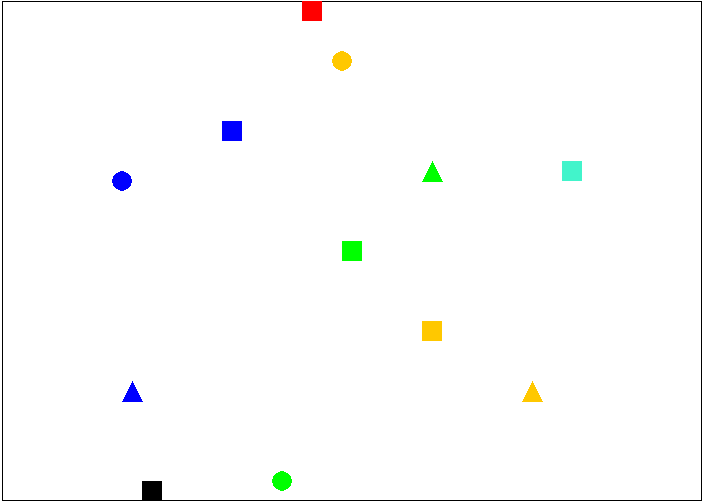
\includegraphics[scale=0.5]{environment}
    \caption{Currently Used Environment}
\end{figure}
\vline

\subsection{Dataset Format and Data Collection}
As mentioned previously, our problem is a multi-label classification problem. So we designed our dataset in accordance. In our dataset, we've a instruction to execute. And which destination is mentioned in this instruction, we collect this information by marking the column of the corresponding destination with value 1. The default value of all columns (for our problem all destination) is 0. The following figure shows how our actual dataset looks like. \\

\begin{figure}[h]
    \centering
    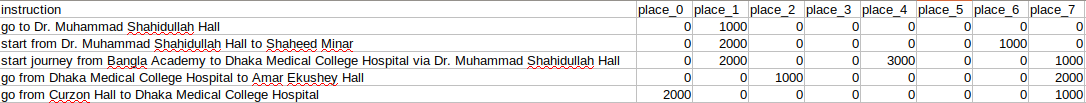
\includegraphics[scale=0.35]{dataset}
    \caption{A Snapshot of used Dataset}
\end{figure}
\vline

\subsection{NLP Pipeline Designing}

The first stage of our work is the designing of a NLP pipeline. The steps associated with designing an ideal NLP pipeline are as follows: \\

\begin{enumerate}
    \item Sentence Segmentation
    \item Word Tokenization
    \item Predicting Parts of Speech for Each Token
    \item Text Lemmatization
    \item Identifying Stop Words
    \item Dependency Parsing
    \begin{enumerate}
        \item Finding Noun Phases
    \end{enumerate}
    \item Named Entity Recognition (NER)
\end{enumerate}
\vline

Now we should focus on a brief discussion of these steps. We consider the sentence: "Go near the red triangle. Wait for three seconds. Then go to green rectangle."\\

\paragraph{Sentence Segmentation}
The first step in the pipeline is to break the text apart into separate sentences. Thus gives us this:
\begin{enumerate}
    \item "Go near the red triangle."
    \item "Wait for three seconds."
    \item "Then go to green rectangle."
\end{enumerate}

\paragraph{Word Tokenization}
Now that we’ve split our document into sentences, we can process them one at a time. The next step in our pipeline is to break this sentence into separate words or tokens. This is called tokenization. This is the result: \\

\begin{tabular}{|p{10cm}}
    "Go", "near", "the", "red", "triangle", "." 
\end{tabular}\\
\vline


Tokenization is easy to do in English. We’ll just split apart words whenever there’s a space between them. And we’ll also treat punctuation marks as separate tokens since punctuation also has meaning.

\paragraph{Predicting Parts of Speech for Each Token}
Next, we'll look at each token and try to guess its part of speech - whether it is a noun, a verb, an adjective and so on. Knowing the role of each word in the sentence will help us start to figure out what the sentence is talking about.\\


We can do this by feeding each word (and some extra words around it for context) into a pre-trained part-of-speech classification model. The part-of-speech model was originally trained by feeding it millions of English sentences with each word’s part of speech already tagged and having it learn to replicate that behavior.\\

After processing the whole sentence, we'll have result like this:
\begin{table}[h]
    \centering
    \begin{tabular}{ccccc}
        Go   & near      & the        & red  & triangle \\
        Verb & Adjective & Determiner & Noun & Noun    
    \end{tabular}
\end{table}

\paragraph{Text Lemmatization}
In English (and most languages), words appear in different forms. When working with text in a computer, it is helpful to know the base form of each word so that we know both sentences are talking about the same concept. In NLP, we call finding this process lemmatization - figuring out the most basic form or lemma of each word in the sentence. The same thing applies to verbs. We can also lemmatize verbs by typically done by having a look-up table of the lemma forms of words based on their part of speech and possibly having some custom rules to handle words that we'ver never seen before.

\paragraph{Identifying Stop Words}
Next, we want to consider the importance of a each word in the sentence. English has a lot of filler words that appear very frequently like “and”, “the”, and “a”. When doing statistics on text, these words introduce a lot of noise since they appear way more frequently than other words. Some NLP pipelines will flag them as stop words —that is, words that you might want to filter out before doing any statistical analysis.

\paragraph{Dependency Parsing}
The next step is to figure out how all the words in our sentence relate to each other. This is called dependency parsing.\\

The goal is to build a tree that assigns a single parent word to each word in the sentence. The root of the tree will be the main verb in the sentence.\\

It’s also important to remember that many English sentences are ambiguous and just really hard to parse. In those cases, the model will make a guess based on what parsed version of the sentence seems most likely but it’s not perfect and sometimes the model will be embarrassingly wrong. But over time our NLP models will continue to get better at parsing text in a sensible way.

\subparagraph{Finding Noun Phrases}
So far, we’ve treated every word in our sentence as a separate entity. But sometimes it makes more sense to group together the words that represent a single idea or thing. We can use the information from the dependency parse tree to automatically group together words that are all talking about the same thing.

\paragraph{Named Entity Recognition (NER)}
The goal of Named Entity Recognition, or NER, is to detect and label the nouns with the real-world concepts that they represent. But NER systems aren’t just doing a simple dictionary lookup. Instead, they are using the context of how a word appears in the sentence and a statistical model to guess which type of noun a word represents.\\

Here are just some of the kinds of objects that a typical NER system can tag: People’s names, Company names, Geographic locations (Both physical and political), Product names, Dates and times, Amounts of money, Names of events.\\

The above mentioned steps are the necessary steps for any ideal NLP Pipeline. But for currently, we weren't able to utilize some steps of this pipeline. For example, Dependency Parsing and Named Entity Recognition wasn't used for our classification task.\\

We pass our input instruction through this Pipeline and get our desired output for our next most important step: classification of the text.\\


\subsection{Classification}
To classify desired destination from our text input, we've used Linear Support Vector Classifier(Linear SVC) classifier. After passing the input instruction through the pipeline we feed this input instruction to our model as X data and corresponding object marker as y data.\\

So the necessary input for the model is as follow:\\
X = ["Go near the blue triangle. Wait for three seconds. Then go to green rectangle."]
y = [0, 1, 0, 0, 0, 0, 0, 0, 0, 0, 1]\\

Corresponding position for blue triangle and red triangle is marked as 1 and all other marked as 0.\\

After the model is trained, if we give another text instruction and ask the model to classify necessary destination marker the model will give us an array with eleven elements, as we've used eleven objects in our environment. In this array all elements are zero except the elements that our model predicted as mentioned in instruction.\\

Once we've the desired output from our model. We marked that location(s) with reward and start navigation process. Navigation process is described in the next section.

\subsection{Action Generation}
For navigating in the environment, our agent has to develop or generate actions for the given instructions. Currently we use the basic reinforcement learning algorithm: Value Iteration to generate actions for the agent.\\

Value Iteration algorithm works in a grid environment where we've one or more rewards and one or more punishments in some grids. According to that reward or punishment we generate value for each action for each grid. The formula associated with value iteration algorithm is as follows:\\

$V^*(s) = \max \sum T(s, a, s')[R(s, a, s')  + \gamma V^*(s')]$\\

An example of a $3 X 3$ grid with optimal policy and optimal values after applying value iteration is given in the following image.\\


\begin{figure}[ht]
    \centering
    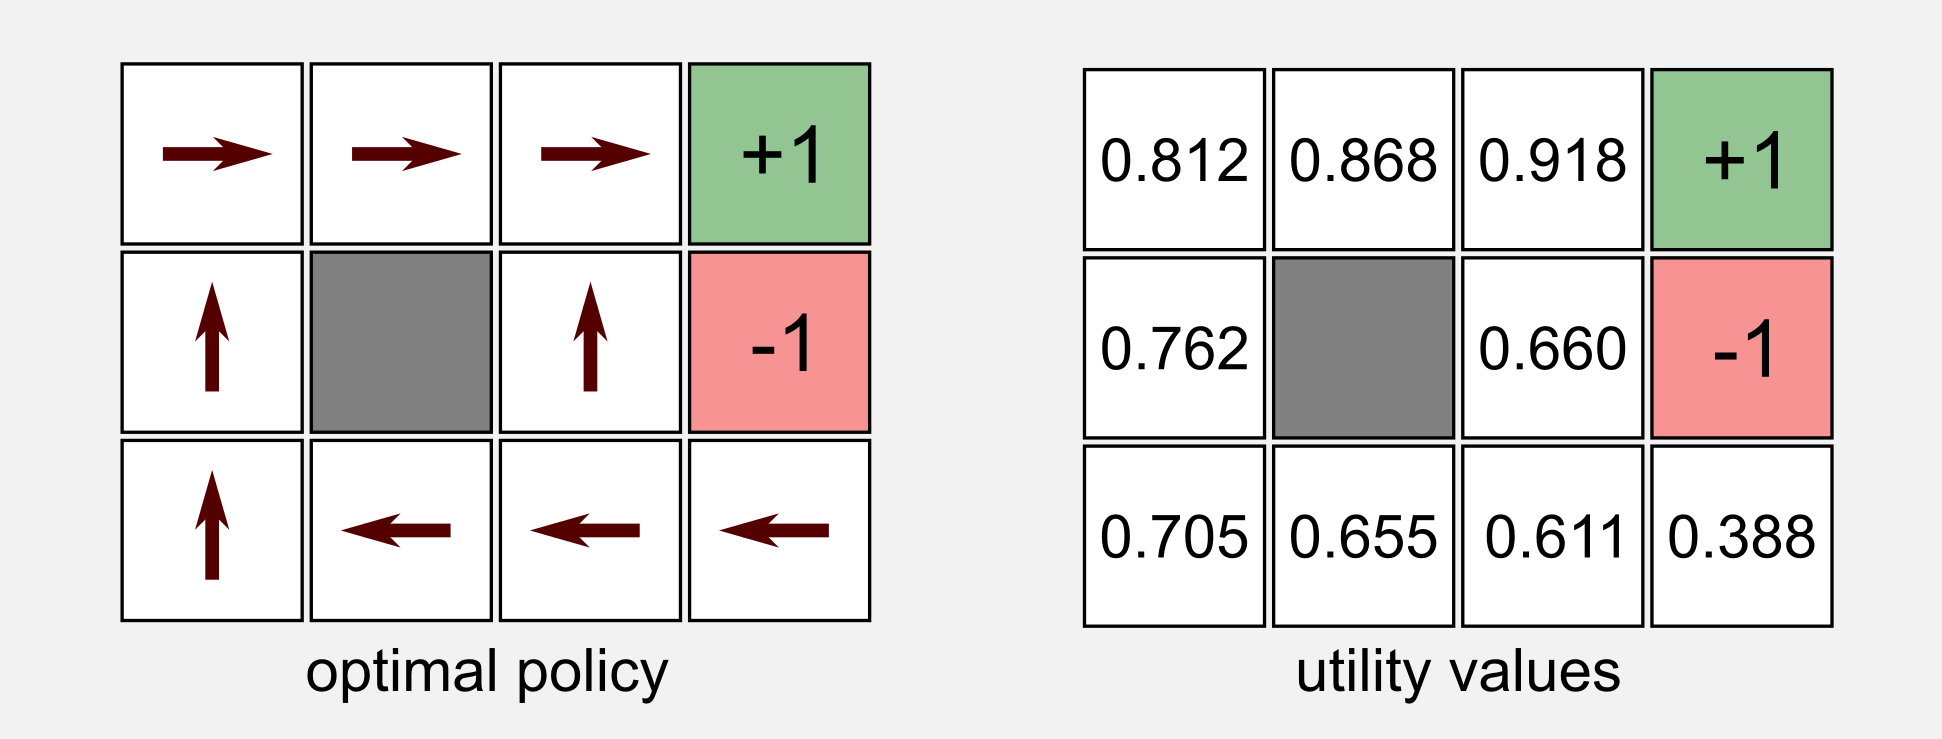
\includegraphics[scale=0.5]{value_iteration}
    \caption{Value Iteration Example}
\end{figure}
\vline

For using the Value Iteration algorithm we split our environment in $25 X 35$ grids. We set reward in grids which is our destinations. We decrease reward value according to the hierarchy or the destination. Similarly we set negative reward in the grid that we should have to avoid.\\

After iterating the algorithm over the whole grid several time we can get the optimal action for each grid. According to this optimal option, agent(robot) will start moving.\\









\section{Expected Work to be Done}

\subsection{Utilizing and Completing the NLP Pipeline}
What pipeline we've already designed is moderately enough for language processing tasks. We didn't use the whole pipeline. From our studies, we acknowledged that we need such Pipeline but we're still not capable of utilizing the whole Pipeline. But we think that the whole Pipeline will be useful if we use some more advance classification model. With the increasing efficiency of our classification model we hope we can utilize the designed Pipeline.\\

We've designed our NLP pipeline for English language. But as our project aims to navigate robot using Bengali language, we've needed some special consideration for Bengali NLP pipeline. We've to convert the whole pipeline such a way that it could process Bengali language.\\


\subsection{Classificaiton}
As our project is focused on classification. By classifying the text we tried to understand that which is our necessary destination in a given instruction. But our model still not capable of performing well. In many cases it can't properly find out desired destination.\\

We used only two models (detail comparison is given in Result section), but we hope to explore some more models that we've noticed in our studies. At the end we hope we would have a strong model with specific hyper-parameters to classify desired destination from the given instruction.\\

\subsection{Environment Designing}
We want to design an environment with real life element like tree, building etc. We want to represent the environment via a graphical interface.\\

Alongside the graphical interface we also demonstrate the environment in real life with some dummy element like toy car or toy tree. We want to synchronize the navigation of real life demo in our graphical interface too.\\

After completing the design of the environment and above mentioned two other steps we hope to have our project ready completely.	
	
	 
		

	
